
%%%%%%%%%%%%%%%%%%%%%%%%%%%%%%%%%%%%%%
%
%     TITLE NAME
%
%%%%%%%%%%%%%%%%%%%%%%%%%%%%%%%%%%%%%%
%\href{https://www.home.me}{homepage.com}
\namesection{Yahya}{Shubbak}{M.Sc. Nanoscience University of Kassel  $\qquad \qquad$ \today}{\contactline
{\href{https://github.com/YahyaShubbak}{NanoYahya}}{\href{https://www.linkedin.com/in/yahya-shubbak-75a537229/}{Yahya Shubbak}}{\href{mailto:y.shubbak@ik.me}{y.shubbak@ik.me}}{\href{tel:+4917680848963}{+49 17680848963}}}

% \namesection{Firstname}{Lastname}{Full Stack Software Engineer}{\contactline{\href{https://www.mazumder.me}{mazumder.me}}{\href{https://www.github.com/sansquoi}{sansquoi}}{\href{https://www.linkedin.com/mazumders}{mazumders}}{\href{mailto:shubham.mazumder@gmail.com}{first.last@email.com}}{\href{tel:+1999999999}{9999999999}}}

%%%%%%%%%%%%%%%%%%%%%%%%%%%%%%%%%%%%%%
%
%     COLUMN ONE
%
%%%%%%%%%%%%%%%%%%%%%%%%%%%%%%%%%%%%%%

\begin{minipage}[t]{0.70\textwidth} 


%%%%%%%%%%%%%%%%%%%%%%%%%%%%%%%%%%%%%%
%     EXPERIENCE
%%%%%%%%%%%%%%%%%%%%%%%%%%%%%%%%%%%%%%

\section{Education}
\runsubsection{Doctorate Research}
\descript{| University of Kassel}
\location{June 2022 – today | Kassel, Germany}
\vspace{\topsep} % Hacky fix for awkward extra vertical space
\begin{tightemize}
%\sectionsep
\item Research topic: \textit{Harnessing close-to-surface transport of magnetic particles in a dynamically transformed magnetic field landscapes for Lab-on-a-chip applications}
\end{tightemize}

\sectionsep

\runsubsection{Master of Science}
\descript{| University of Kassel}
\location{April 2019 – March 2022 | Kassel, Germany}
%\vspace{\topsep} % Hacky fix for awkward extra vertical space
\begin{tightemize}
%\sectionsep
\item Master thesis in nanoscience at the department of atomic and molecular physic, titled \textit{Processing and Characterization of a bi-Stable Sublimable Molecular Spin-Crossover Fe(II)-Complex} 


Graded \textbf{1.15}. Cumulative grade: \textbf{1.3}
\end{tightemize}

\location{September 2019 - October 2020 | València, Spain}
%\vspace{\topsep} % Hacky fix for awkward extra vertical space
\begin{tightemize}
\item Erasmus at the University of València in the master program \textit{Molecular Nanocience and Nanotechnology} combined with the research for the master thesis
\end{tightemize}

\sectionsep

\runsubsection{Bachelor of Science}
\descript{| University of Kassel}
\location{October 2014 – June 2019 | Kassel, Germany}
%\vspace{\topsep} % Hacky fix for awkward extra vertical space
\begin{tightemize}
%\sectionsep
\item Bachelor thesis in nanoscience at the department of atomic and molecular physic, titled \textit{Design and Characterization of a Fiber Adaptation for a Czerny-Turner-Spectrometer with a Position sensitive Detector at the Example of Carbon Emission Lines - Swan Bands}

Graded \textbf{1.86}. Cumulative grade: \textbf{2.2}
\end{tightemize}

\location{September 2016 - May 2017 | Calgary, Canada}
%\vspace{\topsep} % Hacky fix for awkward extra vertical space
\begin{tightemize}
\item Studies abroad at the University of Calgary at the Physics department
\end{tightemize}
\sectionsep

\runsubsection{School Education}
%\descript{| Kassel } 
\\
%\location{September 2011 – July 2014 | High School | Elisabeth-Knipping-Schule Kassel | Abitur 1.8 }
%\location{September 2005 – July 2011 | Middle School | Gesamtschule Fuldatal}
%\location{August 2001 - July 2005 | Elementary School | Wolfsanger/Hasenhecke}
\location{August 2001 – July 2014 | Kassel, Germany }
\begin{tightemize}
\item Abitur (High School Diploma) at the Elisabeth-Knipping-Schule Kassel. 

Cumulative grade: \textbf{1.8}
\end{tightemize}
\sectionsep
\runsubsection{Research stay}\\
\location{April 2022 | Paris, France}
\begin{tightemize}
\item Beamtime at HERMES, Synchrotron facility Soleil
\end{tightemize}
\location{September 2020 | Barcelona, Spain}
\begin{tightemize}
\item Beamtime at BOREAS, Synchrotron facility Alba
\end{tightemize}

\sectionsep

\runsubsection{Conferences} \\
\location{Fall 2022}
\begin{tightemize}
\item DPG Congress of the Condensed Matter Section in Regensburg, Germany, poster presentation


Largest physics congress in Europe with over 4000 visitors from 40 countries and 3600 contributions
\end{tightemize}
\location{Spring 2022}
\begin{tightemize}
\item 20 years CINSaT workshop in Kassel, Germany, poster presentation 


\end{tightemize}
\location{Fall 2021}
\begin{tightemize}
\item CINSaT Fall Colloquium in Kassel, Germany, poster presentation 
\end{tightemize}
\location{Fall 2021}
\begin{tightemize}
\item 84th Annual Meeting of DPG of the Condensed Matter Section, poster presentation
\end{tightemize}
\begin{comment}

%%%%%%%%%%%%%%%%%%%%%%%%%%%%%%%%%%%%%%
%     Projects
%%%%%%%%%%%%%%%%%%%%%%%%%%%%%%%%%%%%%%

%\section{Awards}

%\runsubsection{Scholarship}
%\descript{| Studienstiftung des deutschen Volkes}
%\location{April 2015 - September 2017 | 2 years 6 months}
%\sectionsep

\section{Experience}
\runsubsection{University Research and Teaching} \\
%\descript{| University of Kassel}
\location{November 2021 – April 2022 | 6 months }
\begin{tightemize}
\item Research assistant at the group of Prof. Dr. Arno Ehresmann, University of Kassel \end{tightemize}
\location{February 2020 – May 2020 | 4 months}
\begin{tightemize}
\item Research assistant at the group of Prof. Dr. Eugenio Coronado, University of València 
\end{tightemize}
\location{May 2019 – August 2019 | 4 months}
\begin{tightemize}
\item Research assistant at the group of Prof. Dr. Arno Ehresmann, University of Kassel
\end{tightemize}
\location{October 2018 - February 2019 | 5 months}
\begin{tightemize}
\item Tutor "General Chemistry for Civil- and Enviromental Engineers", University of Kassel
\end{tightemize}
\vspace{\topsep} % Hacky fix for awkward extra vertical space
%\sectionsep
\runsubsection{Research stay}\\
\location{April 2022 | Paris, France}
\begin{tightemize}
\item Beam time at HERMES, Synchrotron facility Soleil
\end{tightemize}
\location{September 2020 | Barcelona, Spain}
\begin{tightemize}
\item Beam time at BOREAS, Synchrotron facility Alba
\end{tightemize}

\runsubsection{Conferences} \\
%\location{Fall 2022}
%\begin{tightemize}
%\item DPG Congress of the Condensed Matter Section in Regensburg, Germany, poster presentation 
%\end{tightemize}
\location{Spring 2022}
\begin{tightemize}
\item 20 years CINSaT workshop in Kassel, Germany, poster presentation 
\end{tightemize}
\location{Fall 2021}
\begin{tightemize}
\item CINSaT Fall Colloquium in Kassel, Germany, poster presentation 
\end{tightemize}
\location{Fall 2021}
\begin{tightemize}
\item 84th Annual Meeting of DPG of the Condensed Matter Section, poster presentation
\end{tightemize}
%%%%%%%%%%%%%%%%%%%%%%%%%%%%%%%%%%%%%%
%     AWARDS
%%%%%%%%%%%%%%%%%%%%%%%%%%%%%%%%%%%%%%

% \section{Awards} 
% \begin{tabular}{rll}
% 2020	     & Finalist & Lorem Ipsum\\
% 2018	     & $2^{nd}$ & Dolor Sit Amet\\
% 2015	     & Finalist  & Cras posuere\\
% \\
% \end{tabular}
% \sectionsep
%%%%%%%%%%%%%%%%%%%%%%%%%%%%%%%%%%%%%%
%
%     COLUMN TWO
%
%%%%%%%%%%%%%%%%%%%%%%%%%%%%%%%%%%%%%%
\end{comment}

\end{minipage} 
\hfill
\begin{minipage}[t]{0.27\textwidth} 

%%%%%%%%%%%%%%%%%%%%%%%%%%%%%%%%%%%%%%
%     SKILLS
%%%%%%%%%%%%%%%%%%%%%%%%%%%%%%%%%%%%%%
\section*{}
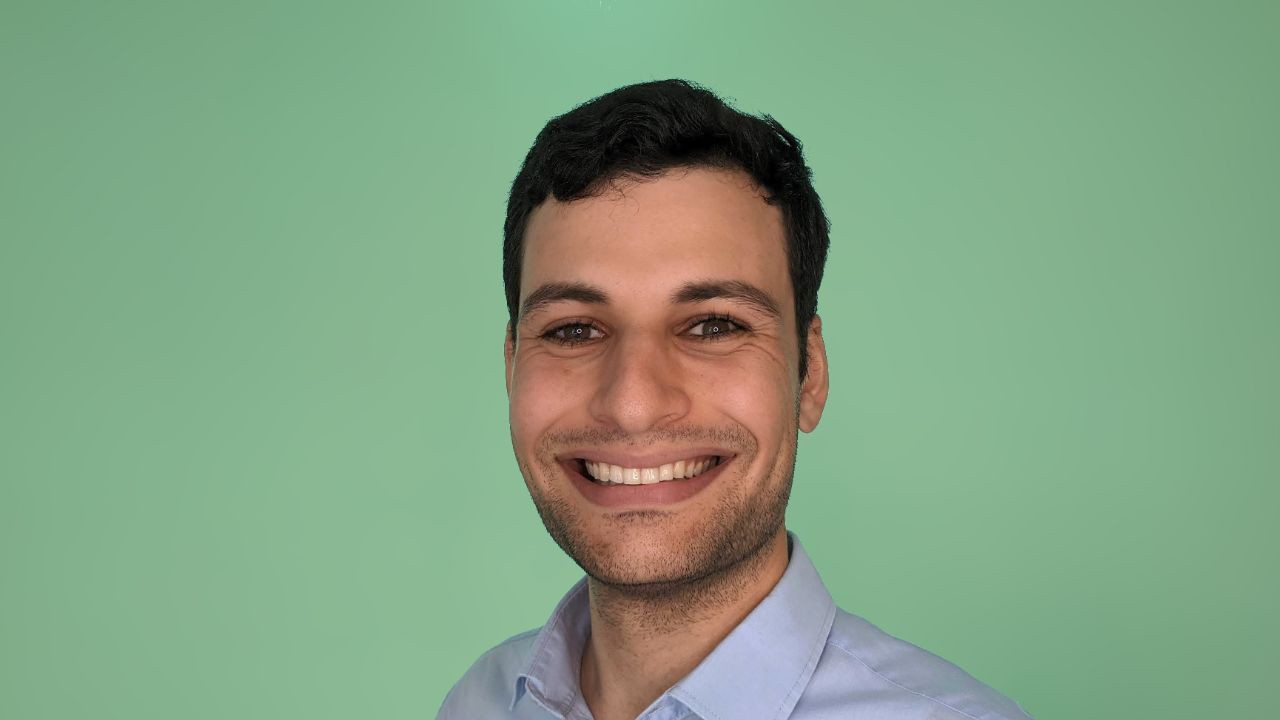
\includegraphics[width=0.8\linewidth,trim={12cm 0 8cm 1cm},clip]{icons/Yahya.jpg}
\section{Awards}

\runsubsection{Scholarship} \\
%\descript{| Studienstiftung des deutschen Volkes}
\location{April 2015 - September 2017 \\ 2 years 6 months}
Studienstiftung des deutschen Volkes

\sectionsep

\section{Skills}
\subsection{Languages}
%\sectionsep
\location{Mother Tongues:}
Arabic \textbullet{} German \\
%\sectionsep
\location{C1 ILETS Certificate:}
English \\
\sectionsep
\location{B1 Level:}
Spanish \\

\sectionsep
\subsection{Programming}
%\sectionsep
\location{Intermediate:}
Python 

\sectionsep

\subsection{Software}
%\sectionsep
\location{Advanced:}
\LaTeX, Inkscape, Jabref, Adobe Lightroom, Microsoft Office \\
\sectionsep
\location{Intermediate:}
Autodesk Inventor, Citavi


% %%%%%%%%%%%%%%%%%%%%%%%%%%%%%%%%%%%%%%
% %     REFERENCES
% %%%%%%%%%%%%%%%%%%%%%%%%%%%%%%%%%%%%%%



%%%%%%%%%%%%%%%%%%%%%%%%%%%%%%%%%%%%%%
%     COURSEWORK
%%%%%%%%%%%%%%%%%%%%%%%%%%%%%%%%%%%%%%

% \section{Coursework}

% \subsection{Graduate}
% Graduate Algorithms \textbullet{}\\ 
% Advanced Computer Architecture \textbullet{}\\ 
% Operating Systems \textbullet{}\\ 
% Artificial Intelligence \textbullet{}\\
% Visualization For Scientific Data \\
% \sectionsep

% \subsection{Undergraduate}

% Database Management Systems \textbullet{}\\
% Object Oriented Analysis and Design \textbullet{}\\
% Artificial Intelligence and Expert Systems \textbullet{}\\
% Scripting Languages and Web Tech \textbullet{}\\
% Software Engineering \\

\end{minipage} 
\newpage
\begin{minipage}[t]{0.70\textwidth} 


%%%%%%%%%%%%%%%%%%%%%%%%%%%%%%%%%%%%%%
%     Projects
%%%%%%%%%%%%%%%%%%%%%%%%%%%%%%%%%%%%%%

%\section{Awards}

%\runsubsection{Scholarship}
%\descript{| Studienstiftung des deutschen Volkes}
%\location{April 2015 - September 2017 | 2 years 6 months}
%\sectionsep

\section{Experience}
\runsubsection{University Research and Teaching} \\
\location{June 2022 – today }
\vspace{\topsep}
\begin{tightemize}
\item Research assistant at the group of Prof. Dr. Arno Ehresmann, University of Kassel 

Enhancing the experimental particle transport setup, utilizing the dark field capabilities of a new microscope
\end{tightemize}
\begin{tightemize}
\item Coordinator for the physics tutorial and exam for electrical engineering students

Design of the exercise sheets and exam, weekly briefing of the tutors to prepare them for the tutorial 
\end{tightemize}
%\descript{| University of Kassel}
\location{November 2021 – April 2022 | 6 months }
%\vspace{\topsep}
\begin{tightemize}
\item Research assistant at the group of Prof. Dr. Arno Ehresmann, University of Kassel

Working in the lab with magnetic thin films and -beads in preparation for the PhD position. Supervision of a research internship was among the responsibilities.
\end{tightemize}
\location{February 2020 – May 2020 | 4 months}
\begin{tightemize}
\item Research assistant at the group of Prof. Dr. Eugenio Coronado, University of València 

Fabricating spin-crossover thin-film devices of different molecular systems for physical investigation   
\end{tightemize}
\location{May 2019 – August 2019 | 4 months}
\begin{tightemize}
\item Research assistant at the group of Prof. Dr. Arno Ehresmann, University of Kassel

Using a self-designed fiber adaptation for a Czerny-Turner-spectrometer with a position sensitive detector, Carbon, Titan and Iron bands were spectroscopically analysed with the astrophysics group of Prof. Dr. Thomas Giesen
\end{tightemize}
\location{October 2018 - February 2019 | 5 months}
\begin{tightemize}
\item Tutor "General Chemistry for Civil- and Enviromental Engineers", University of Kassel

In-person tutoring of the lecture on general chemistry in front of 40+ students.
\end{tightemize}
\vspace{\topsep} % Hacky fix for awkward extra vertical space
%\sectionsep

%%%%%%%%%%%%%%%%%%%%%%%%%%%%%%%%%%%%%%
%     AWARDS
%%%%%%%%%%%%%%%%%%%%%%%%%%%%%%%%%%%%%%

% \section{Awards} 
% \begin{tabular}{rll}
% 2020	     & Finalist & Lorem Ipsum\\
% 2018	     & $2^{nd}$ & Dolor Sit Amet\\
% 2015	     & Finalist  & Cras posuere\\
% \\
% \end{tabular}
% \sectionsep
%%%%%%%%%%%%%%%%%%%%%%%%%%%%%%%%%%%%%%
%
%     COLUMN TWO
%
%%%%%%%%%%%%%%%%%%%%%%%%%%%%%%%%%%%%%%
\end{minipage} 
\hfill
\begin{minipage}[t]{0.27\textwidth} 
\section{References} 
\href{http://ag-ehresmann.de/}{\textbf{Prof. Dr. Arno Ehresmann}, Professor, University of Kassel}
\begingroup
\setbox0=\hbox{

\includegraphics[scale=0.1,trim={0 1cm 0cm 0cm}]{icons/main/mail.png}\hspace{0.1cm}
\href{mailto:ehresmann@physik.uni-kassel.de}{ehresmann@physik.uni-kassel.de} 
}
\parbox{\wd0}{\box0}
\endgroup
\begingroup
\setbox0=\hbox{

\includegraphics[scale=0.1,trim={0 1.25cm -0.4cm 0cm}]{icons/main/phone.png}\hspace{0.1cm}+49 561 804-4060
}
\parbox{\wd0}{\box0}\endgroup
\\
\sectionsep
\href{https://www.linkedin.com/in/navarro-moratalla-efrén-1bb1b4a5/?originalSubdomain=es} {\textbf{Dr. Efrén Navarro Moratalla}, Research Fellow, Group Leader University of València} 
\\
\begingroup
\setbox0=\hbox{

\includegraphics[scale=0.1,trim={0 1cm 0cm 0cm}]{icons/main/mail.png}\hspace{0.1cm}  	\href{mailto:efren.navarro@uv.es}{efren.navarro@uv.es}
}
\parbox{\wd0}{\box0}
\endgroup
\begingroup
\setbox0=\hbox{

\includegraphics[scale=0.1,trim={0 1.25cm -0.4cm 0cm}]{icons/main/phone.png}\hspace{0.1cm}+34 963544181
}
\parbox{\wd0}{\box0}\endgroup
\\
\sectionsep
\href{https://contacts.ucalgary.ca/info/phas/profiles/1-6248004} {\textbf{Dr. Sean Stotyn}, Senior Instructor University of Calgary} 
\\
\begingroup
\setbox0=\hbox{

\includegraphics[scale=0.1,trim={0 1cm 0cm 0cm}]{icons/main/mail.png}\hspace{0.1cm}  	\href{mailto:sean.stotyn@ucalgary.ca}{sean.stotyn@ucalgary.ca}
}
\parbox{\wd0}{\box0}
\endgroup
\begingroup
\setbox0=\hbox{

\includegraphics[scale=0.1,trim={0 1.25cm -0.4cm 0cm}]{icons/main/phone.png}\hspace{0.1cm}+1 403 210-7594
}
\parbox{\wd0}{\box0}\endgroup
\\

\end{minipage} 

